%%%%%%%%%%%%%%%%%%%%%%%%%%%%%%%%%%%%%%%%%%%%%%%%%%%%%%%%%%%%%%%%%%%%%%
%                                                                    %
%       TEMPLATE BÁO CÁO OSG202 - PHIÊN BẢN CẬP NHẬT (CHUẨN NHẤT)     %
%                                                                    %
% Tác giả: Gemini (Hiệu chỉnh dựa trên hình ảnh minh họa APA 7th)     %
% Ngày cập nhật: 20/10/2025                                          %
%                                                                    %
% CÁC CẬP NHẬT QUAN TRỌNG:                                            %
% 1. Trang bìa được định dạng lại khoảng cách cho giống hình ảnh.      %
% 2. Tự động lặp lại tiêu đề bài báo cáo ở đầu trang 2.                %
% 3. Tiêu đề mục cấp 1 (\section) được tự động căn giữa.               %
% 4. Giữ nguyên giãn dòng 1.5 theo yêu cầu của giảng viên.             %
% 5. Hỗ trợ tiếng Việt với XeLaTeX/LuaLaTeX                           %
%                                                                    %
%%%%%%%%%%%%%%%%%%%%%%%%%%%%%%%%%%%%%%%%%%%%%%%%%%%%%%%%%%%%%%%%%%%%%%

% --- PHẦN PREAMBLE: KHAI BÁO CÁC GÓI VÀ THIẾT LẬP ---

\documentclass[12pt]{article}

\usepackage{float}
\usepackage{booktabs}       % Để tạo bảng biểu đẹp hơn
\usepackage{pifont}         % Để dùng ký hiệu checkmark/cross
\usepackage{hyperref}       % Tạo hyperlink cho mục lục và trích dẫn

% --- Các gói cần thiết cho định dạng ---
\usepackage[margin=1in]{geometry}

% --- Sử dụng XeLaTeX/LuaLaTeX cho hỗ trợ Unicode tốt hơn ---
\usepackage{fontspec}
\setmainfont{Times New Roman}
\setsansfont{Arial}

% --- Gói để chỉnh giãn dòng 1.5 ---
\usepackage{setspace}

% --- Gói cho trích dẫn và tài liệu tham khảo chuẩn APA 7th ---
\usepackage[style=apa, backend=biber, sortcites=true]{biblatex}
\addbibresource{bibliography.bib}

% --- Các gói hỗ trợ khác ---
\usepackage{graphicx}
\usepackage{booktabs}
\usepackage{hyperref}
\hypersetup{
    colorlinks=true, linkcolor=black, filecolor=black,      
    urlcolor=blue, citecolor=black,
}

% --- Gói để tùy chỉnh header/footer (cho số trang) ---
\usepackage{fancyhdr}
\pagestyle{fancy}
\fancyhf{} % Xóa tất cả header và footer mặc định
\rhead{\thepage} % Đặt số trang ở góc trên bên phải

% --- Sửa lỗi headheight ---
\setlength{\headheight}{14.5pt}

% --- Gói để căn giữa tiêu đề mục (\section) ---
\usepackage{sectsty}
\sectionfont{\centering} % Đặt tất cả \section căn giữa

% --- Bắt đầu nội dung tài liệu ---
\begin{document}

% --- TRANG BÌA (TITLE PAGE) - ĐÃ CẬP NHẬT ĐỊNH DẠNG ---
\begin{titlepage}
    \thispagestyle{fancy} % Áp dụng kiểu trang có số trang cho trang bìa
    \centering
    
    \vspace*{3\baselineskip} % Đẩy tiêu đề xuống 3-4 dòng từ lề trên
    
    {\Large \bfseries Group Report: Topic 4 – File Systems and Storage Management\par}
    
    \vspace{2\baselineskip} % Thêm 1 dòng trống (tương đương 2\baselineskip trong giãn dòng 1.5)
    
    {\large
        Nguyen Ngoc Phuc - SE203055 \\
        Dam Le Tuan Anh - SE204111\\
        Nguyen Quang Son - SE171738\\
    }
    
    
    {\large FPT University\par} % Thêm Affiliation
    
    
    {\large OSG202 – Operating Systems\par}
    
    
    {\large Le Bao Duy\par}
    
    
    {\large October 24, 2025\par}
    
\end{titlepage}

% --- THIẾT LẬP GIÃN DÒNG 1.5 CHO TOÀN BỘ BÀI ---
\onehalfspacing 

% --- TẠO MỤC LỤC ---
\tableofcontents
\newpage

%%%%%%%%%%%%%%%%%%%%%%%%%%%%%%%%%%%%%%%%%%%%%%%%%%%%%%%%%%%%%%%%%%%%%%
%                      BẮT ĐẦU NỘI DUNG CHÍNH                       %
%%%%%%%%%%%%%%%%%%%%%%%%%%%%%%%%%%%%%%%%%%%%%%%%%%%%%%%%%%%%%%%%%%%%%%

% --- TỰ ĐỘNG LẶP LẠI TIÊU ĐỀ Ở ĐẦU TRANG 2 ---
\begin{center}
    \large \bfseries Group Report: A Comprehensive Analysis of File Systems and Storage Management
\end{center}
\vspace{1\baselineskip} % Thêm một khoảng trống nhỏ sau tiêu đề

\section{Introduction}

Digital information growth is characterizing the 21st century and was never before witnessed. As stated in the seminal works on storage management, newer technologies such as social networks or mobile devices are constantly producing a huge amount of data, creating what has been described as the ``expanding digital universe'' \parencite{EMC2012InformationStorage}.

Therefore, store devices performance control is now the focus issue and most critical bottleneck in contemporary computer system design \parencite{Pokharel2021}. The goal isn’t just to save data, but also organize it, protect and make it easily retrievable. The underlying problem is at the \textbf{file system}, the essential abstraction that mediates between application software on one hand and storage hardware on the other \parencite{Silberschatz2018}. The design and development of file systems is one among many aspects studied in the history of operating system emulation: from the largely retrograde File Allocation Table (FAT) only suitable for early personal computers to the robust, journaling NTFS and ext4, complexity has not been absent enctype. Performance, Reliability, and Advanced Features Every new generation exhibits impressive progress in performance, reliability, and other advanced features to cope with growing needs of the digital age \parencite{Tanenbaum2014}.




To study this important domain to the fullest extent, we formulate the following six leading aims of this paper:

\begin{enumerate}

  \item Describe and discuss the basic ideas of a file system: files, directories, meta-data, and blocks.

  \item Describe and contrast structures of three typical file systems: FAT, ext4, NTFS.

  \item Compare and contrast the main methods used for storage space allocation: contiguous, linked, and indexed.

  \item Study the different disk I/O scheduling algorithms: FCFS, SSTF, SCAN and C-SCAN.

  \item Describe the basic system performance and reliability methods - caching, buffering and logging.

  \item Do an in-depth case study of one actual heavily-used file system in the wild: Windows’ NTFS or Linux’s ext4.

\end{enumerate}

The report is structured as a positive sequence of thought. Theoretical background: Section 2 Theoretical background is focussed on concepts and technologies that are relevant. We also give a fuller comparison and a detailed case study demonstrating the effect of our technique on practical applications in section 3. In Section 4, we discuss the broader implications and trade-offs, and the potential for exploiting contemporary storage technologies. Section 5 concludes the paper, and provides future direction in storage management research.

\section{Background / Literature Review}
%======================================================================
% Section 2.1: Fundamental Concepts
%======================================================================

\subsection{Fundamental Concepts}

An OS needs a consistent interface to read and write data. The file system is the abstraction layer that the OS uses to manage data on physical storage. To appreciate how these convoluted file system structures really work you need to understand a few key elements: the file, the directory, metadata and the block.

\subsubsection{File}
In essence, a \textbf{file} is a group of related records or information, identified by a unique name and stored as a unit \parencite{EMC2012InformationStorage}. From a user's viewpoint, a file is the minimum logical amount of data that can be stored. A file system implements all the necessary functions for you to create, read, write, and delete files. Access to a file is controlled by access permissions, which are assigned by the file's owner and enforced by the operating system \parencite{Silberschatz2018}. Usually a file has a number of attributes associated with it such as its name, its type, location on the storage media, size, protection, and timestamps (creation time, last access time or last modification time).


\subsubsection{Directory}
To manage thousands or millions of files effectively, file systems employ a hierarchical structure called a \textbf{directory}. A directory in essence is a special file that functions as a “container” holding pointers to files or subdirectories \parencite{EMC2012InformationStorage}. Today, all file system implementations keep a pointer map to directories, subdirectories and files in order to build a tree structure enabling users and applications to access the system logically either through absolute or relative paths \parencite{Tanenbaum2014}. 

\subsubsection{Metadata}
Alongside user information managed in the form of files, the file system also has to maintain a large amount of structural information. This set of information is collectively termed \textbf{metadata} – or "data about data" \parencite{EMC2012InformationStorage}. Metadata is extremely important for the file system's integrity and administration.

One classic practical example is the \textbf{inode} in UNIX-like operating systems including Linux. Each directory and file has its own inode. The inode doesn't hold the file or directory's data itself but it does contain all the information about the file including its permissions (read, write, execute), the owner and group IDs, file size, timestamps (last access, last modification), and most importantly an array of pointers to the actual data blocks on the disk where the content of the file is stored \parencite{LinuxJournalInode}. Likewise, the Master File Table (MFT) acts as the nucleus metadata database in the Windows NTFS file system, and each file is represented by an MFT record \parencite{Silberschatz2018}. 

\subsubsection{Block}
At the hardware level a disk is split into addressable units named sectors. But the file system allocates the disk space in larger unit called \textbf{block}. A file system block is the smallest “container” of physical disk space that can be allocated for data, and it is made up of one or more adjacent sectors \parencite{EMC2012InformationStorage}. The block size (e.g. 4KB) is constant during the creation of the file system. Most files are bigger than one block and therefore take up more than one block on a disk. With blocks being added or removed, a file's blocks can become noncontiguous, resulting in \textbf{fragmentation}, which can have an impact on the performance of reading data \parencite{Tanenbaum2014}.

%======================================================================
% PHẦN 2.2: File System Architectures}
%======================================================================


\subsection{File System Architectures}
The file systems have evolved substantially since the early simple forms to complex, dependable, full-featured systems of today. The selection of the file system has a great influence on the performance, compatibility, and data integrity of the whole system. This paper is going to discuss three representative architectures (for major ecosystems) – FAT, ext4, and NTFS. 

\subsubsection{FAT (File Allocation Table)}
Originally presented in 1977 with MS-DOS, the \textbf{FAT (File Allocation Table)} is one of the easiest and most widely used file systems \parencite{Bundele2018}. The layout of a FAT partition is divided in to three areas: a boot sector, the FAT and the data area. The F A T (file allocation table) is a linked list on the disk with each entry corresponding to a cluster in the data area and contains the next cluster of the file or a special end of file marker \parencite{Tanenbaum2014}.

FAT existed in multiple versions over the years, such as FAT12, FAT16, and currently, with the highest spread version being FAT32. Using 32-bit entries in the table allows FAT32 to support up to 2TB partitions and up to 4GB as max file size \parencite{Bundele2018}. Structural simplicity has always been the greatest strength of FAT, although it has many restrictions, including the high fragmentation susceptibility and the lack of modern features (journaling, file-level security, etc.). It Provides You With Almost Universal Compatibility With Different Operating Systems (Windows, Linux, Mac, Android, And More). Therefore, FAT32 is still the most popular file system for portable drive such as USB, flash drive and SD card \parencite{Dhjaku2019}. 

\subsubsection{ext4 (Fourth Extended Filesystem): The Standard for Linux}
Background The ext4 file system is the successor of and a major improvement over the widely used ext2 and ext3 file systems, and is now the default file system for many Linux distributions. A major architectural change was the adoption of extents as the basic flexible block allocation structure replacing the standard block mapping found in ext3. Instead of storing a pointer for each individual block of data (as was done in ext3), an extent is a single very large structure that points to a run of contiguous blocks of data on the disk. This leads to a reduction in fragmentation, better access performance for larger files, and simpler management of metadata \parencite{Dhjaku2019}. 

Besides, ext4 implements a number of other modern features such as delayed allocation, which enables the file system to wait for a number of disc write blocks to be delivered before allocating space on the disk, improving the allocation decisions. Ext4 also improves its journaling through checksums of the journal, enhancing reliability and detecting failures early \parencite{Dhjaku2019}. With its 64-bit support, ext4 can handle volumes up to 1 Exabyte (EB) and files as large as 16 Terabytes (TB) that is sufficient for the requirements of the current large-scale storage.

\subsubsection{NTFS (New Technology File System): The Foundation of Windows}
Originally released in 1993, the NTFS file system was natively architected with centralized features in modern Windows NT family operating systems \parencite{Cunningham2024}. NTFS is based on a revolutionary data structure known as the Master File Table (MFT). MFT is essentially a special file that acts like a database and contains one or more records per file and directory in the partition. Every record contains all the metadata of the file like its name, size, timestamps, and many other attributes. If the file is small enough, even the file content is stored directly inside the MFT record, furry access to the file \parencite{Dhjaku2019, Silberschatz2018}. 

NTFS is better than FAT in every way, because of a bunch of advanced functionalities. It is a fully journaled file system, so after a system crash it can be brought back online quickly with data integrity. Security NTFS has a more granular permission model through the use of Access control lists (ACLs) which allows administrators to specify exactly what rights a user or group have to a file or folder on a per-file/directory basis. Other additions include file-system-level data compression and encryption (EFS), and the Volume Shadow Copy Service (VSS) that enables snapshots CREATION \parencite{Tanenbaum2014}. These traits have established NTFS as a must-have for the Windows platform, especially in servers and enterprise systems.

\subsubsection{Comparative Summary}
To summarize the distinction between the three architectures, the following table \ref{tab:fs_comparison} outlines a detailed comparison with respect to the major technical and performance aspects. The information in this table was drawn from textbooks classics and comparative studies \parencite{Dhjaku2019, Bundele2018}.

 % % --- SẢN PHẨM 2: BẢNG SO SÁNH ---
 
 \begin{table}[H]
     \centering
     \caption{Comparative table of file system structures.}
     \label{tab:fs_comparison}
     \begin{tabular}{@{}llll@{}}
         \toprule
         \textbf{Feature} & \textbf{FAT32} & \textbf{ext4} & \textbf{NTFS} \\ 
         \midrule
         Max File Size     & 4 GB                  & 16 TB                 & 16 EB (theoretically) \\
         Max Volume Size   & 2 TB (up to 16 TB)    & 1 EB                  & 256 TB (practical)    \\
         Journaling        & No                  & Yes                 & Yes                 \\
         Metadata          & Minimal (FAT Table)   & Rich (Inodes)         & Very Rich (MFT)       \\
         Permissions       & Basic (Share-level)   & POSIX                 & ACLs                  \\
         Fragmentation     & High                  & Low (due to Extents)  & Medium                \\
         Performance       & Low                   & High                  & High                  \\
         Ideal Use         & Portable Devices      & Linux Systems         & Windows Systems       \\ 
         \bottomrule
     \end{tabular}
 \end{table}



%======================================================================
% PHẦN 2.3: CÁC PHƯƠNG PHÁP CẤP PHÁT
%======================================================================

\subsection{Allocation Methods}
The Allocation Method is the way the OS allocates and tracks file disk blocks. The selection of the allocation method has an immediate effect on system performance, the wasted space on the storage medium, and the difficulty of managing the files. Three general and classical methods are: contiguous allocation, linked allocation, and indexed allocation \parencite{Silberschatz2018}.

\subsubsection{Contiguous Allocation}
Contiguous allocation mechanisms, require files to be stored in consecutive blocks on the disk. The directory entry for the file needs to hold two numbers only for accounting purposes: the start of the file on the disc (or start of the partition in the case of a swap file) plus the length of the file \parencite{Tanenbaum2014}.

Is performance the whole benefit of this technique? So it provides a very efficient sequential access, since the disk-head is moved only to the first block, and then is read sequentially without further seek motions. Also, access is very fast in a random manner since the location of any block within the file can be determined directly from the starting address \parencite{Fiveable2025}.

but the chief disadvantage of this algorithm is problem of \textbf{external fragmentation}. As files are created and destroyed, this free space on the disk also gets split into a lot of little, non contiguous pieces As a file lives and dies, its chunks are reassembled. This results in the case where the total free space is enough to hold a file, but no contiguous block of free space is. Another problem is difficulty in extending a file once it has been created, since the space next to the file may be taken \parencite{Silberschatz2018}.

\subsubsection{Linked Allocation}
Linked allocation was introduced to address the problem of external fragmentation. In this scheme, each file is a linked list of disk blocks, which are scattered all over the disk. Each block has the data of the file and a pointer to the next block. The directory entry need only store the address of the first block \parencite{Silberschatz2018} .

The primary benefit of this technique is that it completely eliminates external fragmentation and simplifies the process of file resizing, since files do not have to be moved. But it also has some drawbacks. Accessing the i-th block i very slow and inefficient, since to access it you have to go through all the first i-1 blocks. In addition, the space occupied by one pointer per block in file system may be substantial and also a corrupted pointer may cause loss of the rest of the file \parencite{Tanenbaum2014}. A popular version of this scheme is the \textbf{File Allocation Table (FAT)} file system in which the pointers are not stored in the data blocks themselves but instead are centralized in a separate table (the FAT table). This method may enhance random access speed to some extent if the FAT table is kept in memory \parencite{Fiveable2025}. 

\subsubsection{Indexed Allocation}
To overcome the slow random access problem in linked allocation, the concept of indexed allocation is used. The idea is to combine all the pointers of a file into a single block called an \textbf{index block}. Now, the directory entry references this index block. An entry, too, points to a data block of the file \parencite{Silberschatz2018}.

This technique allows good random access since the entire "map" of the file can be read at once by loading the index block in memory. And it is immune to external fragmentation. Nevertheless, it wastes space for tiny files (as a whole block is dedicated to storing just a handful of pointers) and it has a ceiling on file size when considering one index block alone \parencite{IRJMETS2021}. This bottleneck is overcome by modern day file systems (like UNIX) by introducing more sophisticated techniques like \textbf{multi-level indexing}, namely, single, double, and triple indirect pointers to index huge files \parencite{Tanenbaum2014}.

Figure \ref{fig:indexed_allocation_diagram} shows the mapping of a logical address to physical blocks through one index block. 

\begin{figure}[H]
    \centering
    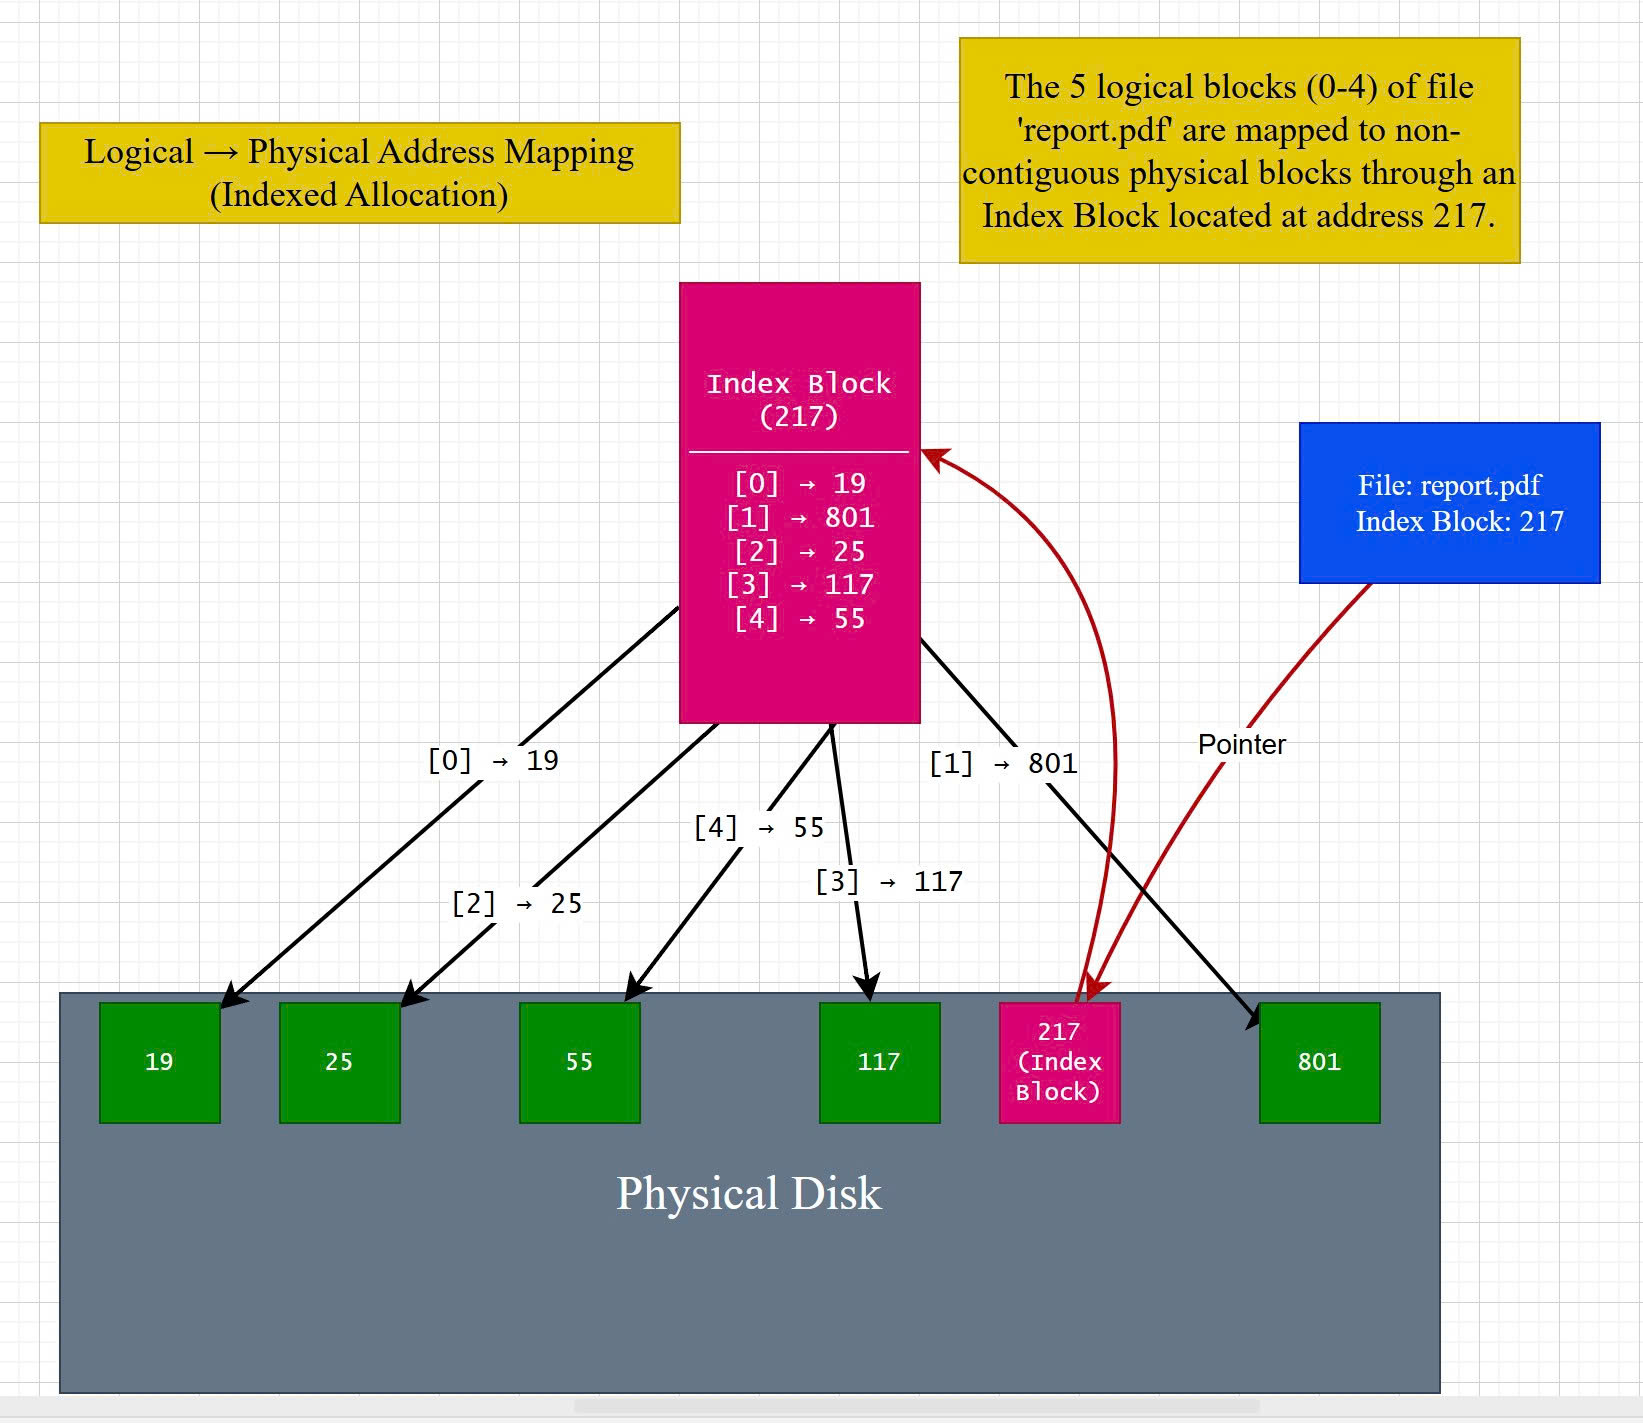
\includegraphics[width=\textwidth]{image/diagram mapping Indexed Allocation.jpg}
    \caption{Logical $\rightarrow$ Physical Address Mapping using Indexed Allocation.}
    \label{fig:indexed_allocation_diagram}
\end{figure}

\subsubsection{Hybrid Approaches and Modern Solutions}
Since all methods have limitations, recent researches have considered hybrid approaches combining the strengths of several methods. One such is the “Hybrid Indexed and Linked List File Allocation System” by Rahman and Siddiqua. This scheme introduces a novel flexible approach: for small size file (e.g., less than 10 blocks) it employs the linked allocation scheme which is to avoid space wastage for a useless index block. When a file exceeds a certain size, the system switches to indexed allocation to provide better random access for large files \parencite{IRJMETS2021}. Such a policy is representative of an attempt to improve allocation performance on the characteristics of each file rather than with one rule for the entire file system. 

%======================================================================
% PHẦN 2.4: LẬP LỊCH TRUY XUẤT ĐĨA
%======================================================================
% % https://calculator.pisqre.com/disk-scheduling
% % https://seektime.app/ : tính vẽ đường này nọ cũng đẹp
% % TODO: BẮT BUỘC THÊM PHẦN TÍNH TOÁN VÀ SƠ ĐỒ GANTT TẠI ĐÂY
% % Dựa trên dàn bài nâng cao, bạn cần thêm một ví dụ cụ thể:
% % - Example Request Queue: 98, 183, 37, 122, 14, 124, 65, 67
% % - Starting position: 53
% % - Tính toán Total Head Movement cho từng thuật toán.
% % - Vẽ sơ đồ Gantt minh họa cho mỗi thuật toán.
% 
\includegraphics[width=\textwidth]{placeholder.png}

\subsection{Disk I/O Scheduling}

One of the primary causes of a performance "bottleneck" for traditional computer systems is the difference in speed between the CPU/main memory and mechanical storage media such as hard disk drives (HDDs) \parencite{Pokharel2021}. For an HDD, data access time has two fundamental parts: seek time—the duration for the read/write head to move to the correct cylinder, and rotational latency—the duration for the sector requested to rotate to the location of the head. Of these, seek time will be the most costly and fluctuating part \parencite{KansalDiskScheduling}. Thus, in a system that supports multitasking where multiple processes concurrently initiate I/O requests, the operating system should have a facility to schedule the completion of the same. It is called disk scheduling, where its foremost aim is to minimize head movement and therefore reduce the average response time as well as increase the system throughput \parencite{GeeksForGeeks2025IO}. The following algorithms are the most widely used methods.

\subsubsection{FCFS (First-Come, First-Served)}
This is the simplest scheduling algorithm, in which I/O requests are serviced in the exact order they arrive. FCFS ensures absolute fairness because no request suffers from starvation. However, it does not perform any optimization regarding head movement. This can lead to very large and inefficient back-and-forth movements of the head across the disk surface, significantly degrading the overall performance of the system \parencite{GeeksForGeeks2025IO}.

\subsubsection{SSTF (Shortest Seek Time First)}
The SSTF algorithm selects the request with the shortest seek time (distance) from the current head position to service next. Essentially, it prioritizes the "closest" requests, regardless of when they arrived. SSTF significantly improves upon FCFS by minimizing the total distance the head travels. However, its major drawback is the potential for starvation: requests at distant cylinders (at the inner or outer edge of the disk) may wait indefinitely if new requests continuously arrive near the current head's position \parencite{GeeksForGeeks2025IO} \parencite{KansalDiskScheduling}.

\subsubsection{SCAN (Elevator Algorithm)}
The SCAN algorithm, also known as the elevator algorithm, works by having the head move from one end of the disk toward the other, servicing all requests in its path. Upon reaching the other end, it reverses direction and repeats the process. SCAN resolves the starvation problem of SSTF because it guarantees it will pass all cylinders. However, it has a slight bias towards the middle cylinders and can cause long waiting times for requests that the head has just passed \parencite{GeeksForGeeks2025IO}.

\subsubsection{C-SCAN (Circular SCAN)}
C-SCAN is an extension of SCAN that is implemented to provide a more balanced waiting time. Similar to SCAN, the head moves from one end of the disk to the other, servicing requests. But when it arrives at the other end, rather than reversing direction, it takes a gigantic "jump" and returns to the starting position and goes on scanning in the same direction. By fulfilling requests in one direction, C-SCAN ensures that requests at the outermost and innermost cylinders get more evenly spaced wait times, eliminating SCAN algorithm bias \parencite{KansalDiskScheduling, GeeksForGeeks2025IO}.

\subsubsection{Quantitative Analysis with an Example}
Assume there is a queue of requests to access the following cylinders: 98, 183, 37, 122, 14, 124, 65, 67. The disk has 200 cylinders (ranging between 0 and 199), and the beginning position of the head is cylinder 53.

\paragraph{FCFS:}
\begin{itemize}
    \item \textbf{Sequence:} 53 \(\rightarrow\) 98 \(\rightarrow\) 183 \(\rightarrow\) 37 \(\rightarrow\) 122 \(\rightarrow\) 14 \(\rightarrow\) 124 \(\rightarrow\) 65 \(\rightarrow\) 67
    \item \textbf{Total Head Movement:} (98-53) + (183-98) + (183-37) + (122-37) + (122-14) + (124-14) + (124-65) + (67-65) = \textbf{640} cylinders.
\end{itemize}

\paragraph{SSTF:}
\begin{itemize}
    \item \textbf{Sequence:} 53 \(\rightarrow\) 65 \(\rightarrow\) 67 \(\rightarrow\) 37 \(\rightarrow\) 14 \(\rightarrow\) 98 \(\rightarrow\) 122 \(\rightarrow\) 124 \(\rightarrow\) 183
    \item \textbf{Total Head Movement:} (65-53) + (67-65) + (67-37) + (37-14) + (98-14) + (122-98) + (124-122) + (183-124) = \textbf{236} cylinders.
\end{itemize}

\paragraph{SCAN (assuming moving towards 199 initially):}
\begin{itemize}
    \item \textbf{Sequence:} 53 \(\rightarrow\) 65 \(\rightarrow\) 67 \(\rightarrow\) 98 \(\rightarrow\) 122 \(\rightarrow\) 124 \(\rightarrow\) 183 \(\rightarrow\) 199 \(\rightarrow\) 37 \(\rightarrow\) 14
    \item \textbf{Total Head Movement:} (199 - 53) + (199 - 14) = 146 + 185 = \textbf{331} cylinders.
\end{itemize}

\paragraph{C-SCAN (assuming moving towards 199 initially):}
\begin{itemize}
    \item \textbf{Sequence:} 53 \(\rightarrow\) 65 \(\rightarrow\) 67 \(\rightarrow\) 98 \(\rightarrow\) 122 \(\rightarrow\) 124 \(\rightarrow\) 183 \(\rightarrow\) 199 \(\rightarrow\) 0 \(\rightarrow\) 14 \(\rightarrow\) 37
    \item \textbf{Total Head Movement:} (199 - 53) + (199 - 0) + (37 - 0) = 146 + 199 + 37 = \textbf{382} cylinders.
\end{itemize}

% TODO: BẮT BUỘC THÊM BIỂU ĐỒ GANTT TẠI ĐÂY
% Bạn có thể dùng công cụ draw.io để vẽ các biểu đồ minh họa chuyển động của đầu đọc cho từng thuật toán,
% sau đó chèn vào file LaTeX dưới dạng hình ảnh.


%======================================================================
% PHẦN 2.5: CÁC KỸ THUẬT TĂNG HIỆU NĂNG VÀ ĐỘ TIN CẬY (PHIÊN BẢN NÂNG CAO)
%======================================================================

\subsection{Performance \& Reliability Techniques}
In addition to optimizing the physical access order, the operating system also implements techniques at the logical layer to enhance performance and ensure data integrity. Three of the most important and popular mechanisms in modern file systems are caching, buffering, and journaling.

\subsubsection{Caching and Buffering}
Although often used interchangeably, buffering and caching are two distinct concepts with different objectives aimed at addressing the I/O performance bottleneck.

\textbf{Buffering} is a technique that uses a buffer (a block of memory) to store data temporarily as it is being transferred from one device operating at a different rate to another. Its primary purpose is to "smooth" data flow and allow processes to continue without having to wait for the physical I/O operation to complete. For example, when an application is performing a write operation, the data can be duplicated into the kernel buffer and the system call will return at once. The kernel will thereafter schedule to write the data out of the buffer to the disk in the background. The buffer data is the original data which is held pending for processing and would typically exist only for a short period of time \parencite{GeeksForGeeks2025BufferCache}.

On the other hand, \textbf{caching} is the act of \textit{duplicating} a heavily used portion of data from a slow storage device (like an HDD) to a quicker memory area (like RAM). Caching is a bid to reduce future \textit{read} access latency. When a read request is made, the system first checks the cache. If the data is in the cache (a cache hit), it is displayed immediately without needing to access the slow device. Otherwise (a cache miss), the data is loaded from the slow device, displayed for the request, and simultaneously a copy of it is stored in the cache to serve future accesses \parencite{GeeksForGeeks2025BufferCache}. Both these mechanisms are usually combined into a single memory management system by the majority of modern operating systems, usually called a \textbf{unified page cache}, to allocate dynamically memory among processes and I/O operations of the file system \parencite{Silberschatz2018}.

\subsubsection{Journaling}
One of the largest problems a file system has is to be in a stable state during an immediate failure, say a power failure or system crash. A simple logical operation such as file deletion can be many individual physical writes to metadata (e.g., marking a bitmap, updating an inode, updating directory entries).. If something goes wrong between these operations, the file system will be in an inconsistent state, and this inconsistency can lead to data loss or storage leaks of space \parencite{LibreTextsJournaling}. Recovery of an inconsistent file system by commands like fsck typically takes very much time because it needs to scan the entire metadata structure of the disk.

In order to solve this problem, modern file systems use a method called journaling, or write-ahead logging. The idea is simple: before writing the changes into the underlying file system structure, a description of the "intent" of the changes is written to a special area called the \textbf{journal}. It is only when this transaction has been safely recorded in the journal and marked as committed that the system initiates the \textbf{checkpointing} process—i.e., writing the actual changes to their permanent residence. On a crash, after rebooting, the system only needs to read the journal and "replay" those transactions that were committed but didn't complete checkpointing to bring the file system to a consistent state very quickly \parencite{Prabhakaran2005journaling, Jones2008Anatomy}.

Journaling file systems typically implement three different operating modes, which represent the trade-off between performance and the level of data protection:

\begin{itemize}
    \item \textbf{Writeback Mode:} This is the highest-performance but riskiest mode. In this mode, only metadata is written to the journal. The file's data is written directly to its permanent location without any synchronization with the metadata write. This means the metadata can be written before or after the data. If a crash occurs, the file system can recover to a consistent metadata state, but the file's data might be old or contain garbage data \parencite{Jones2008Anatomy}.

    \item \textbf{Ordered Mode:} This is the default for most Linux filesystems (ext3 and ext4) and provides a good compromise between performance and security. Similar to writeback, only metadata is actually written into the journal. This mode does, however, have a strict write ordering: data in the file \textit{must} be written to its ultimate destination \textit{before} its corresponding metadata is written into the journal. This structure is in the form that metadata will never point to garbage or unwritten data blocks and therefore prevent corruption of the data during recovery, though the most recent modifications could be lost. \parencite{Prabhakaran2005journaling}.

    \item \textbf{Data Mode (Full Data Journaling):} This is the safest but slowest mode. Under this mode, both the file's \textbf{metadata and data} are written to the journal before checkpointing. That means each data block is written twice: once to the journal and the other to the destination. This mode gives the highest level of consistency; after a crash, the file will either be in its new or old state completely. However, this double-writing significantly reduces the system's write throughput \parencite{Jones2008Anatomy}.
\end{itemize}



%======================================================================
% PHẦN 3: CASE STUDY NTFS
%======================================================================

\section{Analysis \& Case Study: NTFS Deep Dive}

%======================================================================
% PHẦN 3.1: PHÂN TÍCH SO SÁNH TỔNG HỢP
%======================================================================

\subsection{Comparative Analysis}
After surveying the theoretical concepts and basic architectures of the three representative file systems in Section 2, this section will proceed to synthesize and directly compare their characteristics based on the critical criteria of performance, reliability, security, and practical use cases. This analysis will highlight the trade-offs between the designs and lay the groundwork for the in-depth case study on NTFS.

\subsubsection{Performance Comparison}
The performance of a file system is highly dependent on how it manages block allocation and metadata. Based on their architectures, we can compare the theoretical performance of FAT32, ext4, and NTFS in the following scenarios:

\begin{itemize}
    \item \textbf{Sequential Access:} Both NTFS and ext4 exhibit superior performance in this regard. ext4 is utilizing the \textbf{extents} feature, which allows it to allocate large, consecutive sets of blocks, significantly minimizing head movement \parencite{Dhjaku2019}. NTFS is likewise employing clever allocation algorithms for storing large files as contiguous as possible. FAT32, being based on a linked list, is highly prone to fragmentation, and reading a large, sequential file can entail many costly seek operations.

    \item \textbf{Random Access:} Index-based file systems like ext4 and NTFS excel here. The inode structure with its multi-level pointers in ext4 and the centralized MFT architecture of NTFS allow the system to quickly locate any data block of a file with just a few metadata lookups. FAT32, once again, falls short because accessing a block in the middle of a file requires traversing the chain of pointers from the beginning \parencite{Silberschatz2018}.

    \item \textbf{Handling small files:} NTFS has a unique advantage with very small files thanks to its \textbf{resident data} feature. If a file's data is small enough, it can be stored directly inside that file's MFT record, completely eliminating the need to access external data blocks and providing extremely fast access speeds \parencite{Tanenbaum2014}. ext4 also handles small files efficiently by attempting to group them into the same block group to increase locality.

    \item \textbf{Handling large files:} The 4GB file size limit of FAT32 makes it unsuitable. Both ext4 and NTFS support extremely large file and volume sizes, up to terabytes and exabytes, respectively, effectively meeting modern storage demands \parencite{Dhjaku2019}.
\end{itemize}

\subsubsection{Security and Reliability}
Regarding reliability and security, the differences between the file systems are very distinct.
\begin{itemize}
    \item \textbf{Reliability:} The most significant advantage of ext4 and NTFS over FAT32 is that they support \textbf{journaling}. As discussed in Section 2.5.3, the journaling mechanism enables the file system to recover quickly to a consistent state after an unanticipated crash, with little opportunity for corruption of metadata structures and a great reduction in disk check (fsck) time at reboot \parencite{Prabhakaran2005journaling}. FAT32 lacks this mechanism, making it more vulnerable to errors and data loss.
    \item \textbf{Security:} FAT32 only has minimal security features at the share level. ext4 and NTFS were designed for multi-user OSes though. ext4 implements the traditional UNIX \textbf{POSIX} permission model to show access rights to three types of users: the owner, group, and others. NTFS, on the other hand, is based on a completely different, more complex and more powerful concept known as \textbf{Access Control Lists (ACLs)}. With ACL is possible to grant and revoke individual permissions (read, write, execute, delete, etc.) to users and groups over a file, or directory, with a granularity not achievable by standard UNIX permissions \parencite{Bundele2018}.
\end{itemize}


\subsubsection{Use Case Scenarios}
From the analysis above, the role of each file system in different environments is clearly defined:
\begin{itemize}
    \item \textbf{FAT32:} Although technologically obsolete, its simplicity and near-universal compatibility make FAT32 (and its successor, exFAT) the number one choice for portable storage devices that require data exchange between different platforms, such as USB flash drives and SD cards.

    \item \textbf{ext4:} As the native file system of the Linux ecosystem, ext4 is the default choice for almost everything, from enterprise servers and desktop computers to embedded devices running Linux. It provides an excellent balance of performance, reliability, and stability in an open-source environment.

    \item \textbf{NTFS:} As the indispensable foundation of the Windows operating system, its rich set of enterprise features, including ACL security, encryption, data compression, and robust recovery capabilities, makes NTFS the default choice for system and data drives in Windows environments, especially for workstations and servers that demand high reliability and manageability.
\end{itemize}

With a general comparative basis established, the report will now proceed with an in-depth case study of the NTFS architecture to illustrate the concepts that have been discussed in greater detail.


%======================================================================
% PHẦN 3.2: CASE STUDY: PHÂN TÍCH CHUYÊN SÂU VỀ NTFS (ĐÃ SỬA LỖI)
%======================================================================

\subsection{Case Study: A Deep Dive into the New Technology File System (NTFS)}

\subsubsection{Introduction}
What started as a inquisitive rookie can pretty easily turn into a scorning veteran as you learn the history of the filthy New Technology File System (NTFS) – a was Microsoft too busy to read and coded from the ground up air humidifier the nice old FAT? To meet the increasing demands of enterprise environments for more performance, reliability, security, and the support of large capacity drives, the architecture of the New Technology File System (NTFS) was designed to provide a solid storage infrastructure \parencite{Shafiei2012}. Now, the NTFS became the default and the indispensable file system for all new Windows OS. 

\subsubsection{Core Architecture: The Master File Table (MFT)}
NTFS architecture is based on a single design principle:  \textit{"everything on the volume is a file"} \parencite{Shafiei2012}. At the core of this is a special file, called \textbf{\$MFT} the Master File Table. Essentially, the MFT is a relational database with a minimum of one record -- typically 1024 bytes -- for each file and directory on the volume \parencite{HarvardCS161Journaling}.

Each MFT record has a set of attributes, which together fully describe the corresponding file or directory. These attributes are basic metadata such as \texttt{\$STANDARD\_INFORMATION} (timestamps and ownership) and \texttt{\$FILE\_NAME}, and a very special one called \texttt{\$DATA} \parencite{Shafiei2012}. One of the most obscure performance enhancements in NTFS involved its management of the \texttt{\$DATA} attribute:

\begin{itemize}
    \item \textbf{Resident Data:} For very small files, instead of being stored in a separate block on the disk, the entire contents of the file is stored directly as an attribute of $DATA$ within the MFT record itself. This completely removes a disk access operation, which leads to extremely high speed reading of small files \parencite{CIRCL2023}.
    
    \item \textbf{Non-resident Data:} If the data of a file does not fit within the MFT record, then it is turned into a non-resident form. Here, the \texttt{\$DATA} attribute does not contain the data itself but instead points to "extents" (or runs) of clusters on the disk where the data lives \parencite{HarvardCS161Journaling}.
\end{itemize}

\subsubsection{Analysis of Advanced Features}
The power of NTFS – over and above its MFT architecture – also comes from its wealth of native enterprise capabilities.

\paragraph{A. Journaling and Recovery (\texttt{\$LogFile}):}
NTFS is a complete journaling file system, ensuring the consistency of the volume even in the event of a sudden crash. This mechanism is implemented through a special metadata file named \textbf{\texttt{\$LogFile}} \parencite{Shafiei2012}. Unlike ext3, which uses "physical logging" (writing the entire modified metadata block), NTFS implements a more sophisticated form of journaling called \textbf{operation logging} (or redo/undo logging). In this model, the journal does not record the entire data block but only the logical operations that describe the change ("redo") and how to reverse that change ("undo") \parencite{HarvardCS161Journaling}. When a transaction is committed, the operating system applies the changes. If the system crashes, during recovery, NTFS scans the \texttt{\$LogFile}, "redoing" completed transactions and "undoing" incomplete transactions, ensuring the file system's metadata is quickly restored to a consistent state.

\paragraph{B. Security: Access Control Lists (ACLs):}
NTFS offers a very flexible and fine-grained security model through \textbf{Access Control Lists(ACLs)}. Every file and folder in an NTFS volume has an ACL, which is basically a list of \textbf{Access Control Entries (ACEs)}. Each ACE designates a user or group and a collection of rights (Read, Write, Execute, etc.) that can be \textit{Allowed} or \textit{Denied} \parencite{SettingAccessControlLists}. This Discretionary Access Control (DAC) model permits admins to fine-tune their access controls at a much finer granularity than the three-level POSIX/Linux model (the "owner," the "group," and "others"). One very important rule in NTFS is that a "Deny" ACE always takes precedence over an "Allow" ACE, which means you can use the "Deny" to really lock down a resource in a very powerful way \parencite{Allison1998}. 

\paragraph{C. Other Enterprise Features:}
\begin{itemize}
    \item \textbf{Volume Shadow Copy Service (VSS):} This is a powerful framework that allows for the creation of point-in-time consistent "snapshots" of a volume, even while the files on it are in use. VSS coordinates between applications, the file system, and hardware providers to temporarily freeze write operations, create the snapshot, and then resume operations. This mechanism (often using a copy-on-write technique) is the foundation for features like online backup and System Restore in Windows \parencite{MicrosoftVSS}.
    \item \textbf{Encryption and Compression:} NTFS supports data encryption and compression at the file system level, transparently to the user. The \textbf{Encrypting File System (EFS)} allows users to encrypt files/folders using a public key encryption mechanism, ensuring that only that user can decrypt the data \parencite{WafaTech2025EFS}. The compression feature, on the other hand, helps save disk space by automatically compressing data when it is written and decompressing it when it is read.
\end{itemize}

\subsubsection{Evaluation and Limitations}

\textbf{Strengths:} The NTFS architecture clearly demonstrates superiority in reliability through journaling, robust security with ACLs, and flexible performance, handling both small (with resident data) and very large files well. Its rich set of enterprise features like VSS and EFS makes it a solid platform for demanding environments.

\textbf{Weaknesses:} The complexity of the MFT and the enhanced functionality of the MFT records and attributes generate massive metadata overhead compared to traditional file systems. Still, the biggest roadblock in ensconcing NTFS as the universal file system in a multi-platform world is compatibility. While NTFS partitions are readable in other operating systems such as Linux and macOS, writing data with stability and high efficiency requires the use of third party drivers (e.g., NTFS-3G), which are normally a result of reverse engineering and may not attain the same level of performance of that of the native driver on Windows \parencite{Dhjaku2019}. 

%======================================================================
% PHẦN 4: BÀN LUẬN (DISCUSSION)
%======================================================================

\section{Discussion}
Theoretical studies and case studies have shown a multi-faceted view of the system of file and storage management. Clearly, there is no “universal” solution that can be applied in all situations; rather, the best decision always requires a balancing of the trade-offs in performance, reliability, cost, and compatibility.

\subsection{Key Findings Interpretation and Design Trade-offs}
This implies that conventional file systems have evolved with elegant mechanisms for maintaining consistency and good performance. Journaling is a case in point: it is a game-changer for reliability, but the technique inherently doubles the write workload for metadata operations — and sometimes for user data, too \parencite{Lu2013Extending}. This trade-off,although acceptable on HDDs, is becoming more pronounced on   modern storage devices. Similarly, allocation schemes also strike a balance between accessibility speed and space utilization; indexed allocation is preferred because of its flexibility.

\subsection{The Impact of Modern Storage: SSDs and New Challenges}
The appearance of solid-state drives (SSDs) changed the hypervisor cost model of storage management. Physical aspects of NAND flash memory, such as the lack of moving mechanical parts, have made legacy disk scheduling algorithms (SCAN, C-SCAN, LOOK) based on the observation that access time to any logical block is nearly constant, obsolete.
But SSD architecture present new and more complex problems that file system must handle while in HDD you may view your data as never being able to be overwritten. Instead, to be written to once more, memory cells (pages) have to be erased before they can be written to again, and this erasure has to be performed on much larger levels of granularity, called "blocks" (cf. \parencite{Viking2017AN0035, Lu2013Extending}).This constraint is the source of two paramount issues:

\begin{itemize}
    \item \textbf{Write Amplification (WA):} The amount of data written to a flash memory exceeds the amount of data the host requested to be written. The major factor is the \textbf{garbage collection (GC)} process, that the SSD controller needs to read valid pages of a block, then copy them to a new block, and finally erase the old block to complete this process. As a result, a small logical write can translate into a number of physical read and write operations, severely impacting performance as well as the lifetime of the drive (expressed in DWPD or TBW) \parencite{Viking2017AN0035}. Factors like random writes, low free space, and absence of the TRIM instruction all greatly raise the WA value.
    \item \textbf{Wear Leveling:} The quantity of information written to a flash memory is greater than the data the host actually wants to write. The major factor is the \textbf{garbage collection (GC)} process, in which, the SSD controller reads valid pages of a block, copies them to a new block, and then erases the old block to finalize this process. Consequently, a small logical write can trigger multiple physical read and write operations, which not only degrades performance but also shortens the drive's endurance (lifespan), measured in DWPD or TBW \parencite{Viking2017AN0035}. The WA factor is significantly worsened by conditions such as random writes, low free space, and the lack of the TRIM command.
\end{itemize} 

Traditional file systems with journaling and metadata updates so frequently can exacerbate write amplification \parencite{Lu2013Extending}. There is a more subtle problem with the \textbf{FLUSH} command meant to render data durably written from a device’s buffer to the storage medium. Today’s SSDs, on the other hand, have huge DRAM buffers and a single “lump-sum” FLUSH command can evoke writing an unrelated gigabytes of data, which severely degrade responsiveness of essential tasks and increases long tail latency, especially on multitasking environments \parencite{Yeon2018RFLUSH}. This indicates that (OS/FS) SE and (SSD controller) HW coop. will become even more critical to maximize the performance.

%======================================================================
% PHẦN 5: KẾT LUẬN (CONCLUSION)
%======================================================================

\section{Conclusion}
The present report covers the basics and advanced features of OS file and storage management. Through theoretical analysis, architectural comparison and a case study, the stated objectives at the beginning have been systematically reached. 

\subsection{Summary of Findings}
The report covers all six core topic demands, beginning by defining basic concepts, describing and comparing file system structures and space allocation, over I/O scheduling algorithms, to file system optimization techniques, and finally to a comprehensive case study on NTFS. The two required deliverables, the Logical-to-physical mapping diagram and the Comparative table of file systems, have been incorporated and presented in the report.

\subsection{Broader Implications and Future Outlook}
The results show that storage management is undergoing a fundamental transformation, motivated by hardware technology evolution. File systems can no longer be considered a completely isolated abstraction layer above the device. Rather, the future is going to entail more cooperation between the operating system and the storage controller.

Next generation file systems are spearheading this trend by developing features to effectively deal with the problems of scale and data integrity in the new storage media.
\begin{itemize}
    \item \textbf{ZFS and Btrfs} have received wider acceptance because of their groundbreaking capabilities. Both leverage a \textbf{copy-on-write (CoW)} technique, which greatly enhances snapshot and cloning production. More importantly, they employ \textbf{checksums} for both data and metadata at every layer, enabling silent data corruption to be automatically detected and, if run in redundant setups (like mirroring or RAID-Z), repairs can be automatically attempted. They also combine volume and file system management for increased flexibility \parencite{Nfina2025BtrfsZFS}.
    \item \textbf{ReFS (Resilient File System)} of Microsoft, which also follows the same philosophy and is supposed to replace NTFS as the file system for servers where integrity and resiliency is paramount. ReFS relies on "integrity streams" which allows for data to be validated and auto-corrected on ReFS when used with Storage Spaces. Features such as block cloning and sparse VDL are also much faster for virtual machine operations clearly prioritizing modern workloads \parencite{Microsoft2025ReFS}.
\end{itemize}
These technologies point to a future in which storage management is not only faster but also more intelligent, flexible and, perhaps most important of all, more reliable, in that it will be able to self-protect its data from the hardware and software failures of the day. 






% --- PHẦN TÀI LIỆU THAM KHẢO ---
\newpage
\printbibliography[title={References}]

% % --- PHẦN TUYÊN BỐ SỬ DỤNG AI ---
% \newpage
% \section*{AI Usage Statement}
% % Viết tuyên bố sử dụng AI của nhóm bạn tại đây.
% Our team used AI tools (ChatGPT, Claude) for the following purposes: (1) Grammar and spelling checking, and (2) Explaining complex technical concepts during the research phase. All core content, analysis, diagrams, and conclusions were developed independently by team members through studying primary sources including OS textbooks, technical documentation, and academic papers. No AI-generated text was directly copied into the report.

\end{document}